\documentclass[a4paper]{article}

\usepackage[T2A]{fontenc}
\usepackage[utf8]{inputenc}
\usepackage[russian]{babel}
\usepackage{graphicx}
\usepackage{float}
\usepackage{mathtools}
\usepackage{wrapfig}
\usepackage{amsfonts, amssymb, amsmath, latexsym}
\usepackage{nicefrac}
\usepackage{hhline}
\usepackage{multirow}
\usepackage[colorlinks=true,linkcolor=blue,citecolor=blue]{hyperref}       % hyperlinks
\usepackage{nicefrac}       % compact symbols for 1/2, etc.
\usepackage{nameref}
\usepackage{booktabs}       % professional-quality tables
\usepackage{algorithm}
\usepackage{algpseudocode}
\usepackage{xcolor, colortbl}
\usepackage{etoolbox}

% \graphicspath{ {./} }

\usepackage[verbose=true,letterpaper]{geometry}

\newgeometry{
    textheight=25cm,
    textwidth=18cm,
    top=2.5cm,
    headheight=12pt,
    headsep=10pt,
    footskip=1cm,
    marginparwidth=15pt
}

%\usepackage{showframe} 

\usepackage{epigraph}
\usepackage{amsmath,amsfonts,amssymb,amsthm,mathtools, mathrsfs}
\usepackage{amsthm}

\title{Работа 4.3.2 \\ Дифракция света на ультрозвуковой волне в жидкости}
\author{Шарапов Денис, Печин Максим, Б05-005}
\date{}

\usepackage{fancyhdr}
\pagestyle{fancy}
\fancyhf{}
\rhead{Работа 4.3.2}
\lhead{}
\cfoot{\thepage}
\usepackage{subcaption}
\usepackage[font={small}]{caption}

\begin{document}

    \maketitle
    % \tableofcontents
    % \newpage
    
\section{Аннотация}

\noindent\textbf{Цель работы:} изучить дифракцию света на синусоидальной акустической решётке, провести наблюдения на фазовой решётке методом тёмного поля. \smallskip
 
\noindent \textbf{В работе используются:} оптическая скамья, осветитель, длиннофокусные объективы, кювета с жидкость, кварцевый излучатель с микрометрическим винтом, генератор ультразвуковой частоты, линза, вертикальная нить на рейтере, микроскоп.

\section{Результаты измерений и обработка данных}

\subsection{Исследование по дифракционной картине}

Оценим \emph{по порядку величины} скорость звука как удвоенное расстояние между наиболее чёткими дифракционными картинами:
$$n = 67 \;\;\text{дел},$$
$$\lambda \approx 67\cdot10\cdot2=1340 \;\; \text{мкм},$$
$$v = \lambda \cdot \nu \approx 1840 \;\; \text{м/с}.$$
Эта величина не является точной, т. к. оценка проводилась по факту наибольшей видимости, поэтому подсчёт погрешностей не имеет смысла.

\begin{table}[!ht]
    \centering
    \caption{Результаты измерения положений дифракционных максимумов}
    \begin{tabular}{|c|cccc|c|}
    \hline
    \multirow{2}{*}{$\nu,$ МГц} & \multicolumn{4}{c|}{$x_m$, мкм}                                                               &       \\ \cline{2-6} 
                                & \multicolumn{1}{c|}{$0$} & \multicolumn{1}{c|}{$+1$}  & \multicolumn{1}{c|}{$-1$}   & $+2$  & $-2$  \\ \hline
    $1,4570$                    & \multicolumn{1}{c|}{$0$} & \multicolumn{1}{c|}{$196$} & \multicolumn{1}{c|}{$-172$} & $384$ & $344$ \\ \hline
    $2,1515$                    & \multicolumn{1}{c|}{$0$} & \multicolumn{1}{c|}{$272$} & \multicolumn{1}{c|}{$-260$} & $-$   & $-$   \\ \hline
    $4,3971$                    & \multicolumn{1}{c|}{$0$} & \multicolumn{1}{c|}{$584$} & \multicolumn{1}{c|}{$-540$} & $-$   & $-$   \\ \hline
    \end{tabular}
\end{table}

\begin{table}[!ht]
    \centering
    \caption{Результаты измерений скорости звука}
    \begin{tabular}{|c|c|c|c|}
    \hline
    $\nu$, Мгц & $1,4570$      & $2,1515$      & $4,3971$      \\ \hline
    $k$        & $182 \pm 3$   & $266 \pm 4$   & $562 \pm 12$  \\ \hline
    $v$, м/с   & $1430 \pm 20$ & $1450 \pm 20$ & $1400 \pm 30$ \\ \hline
    \end{tabular}
    \end{table}


\noindent График зависимости $x_m(m)$ приведён на рис. 1.
\begin{figure}[!ht]
			\begin{center}
				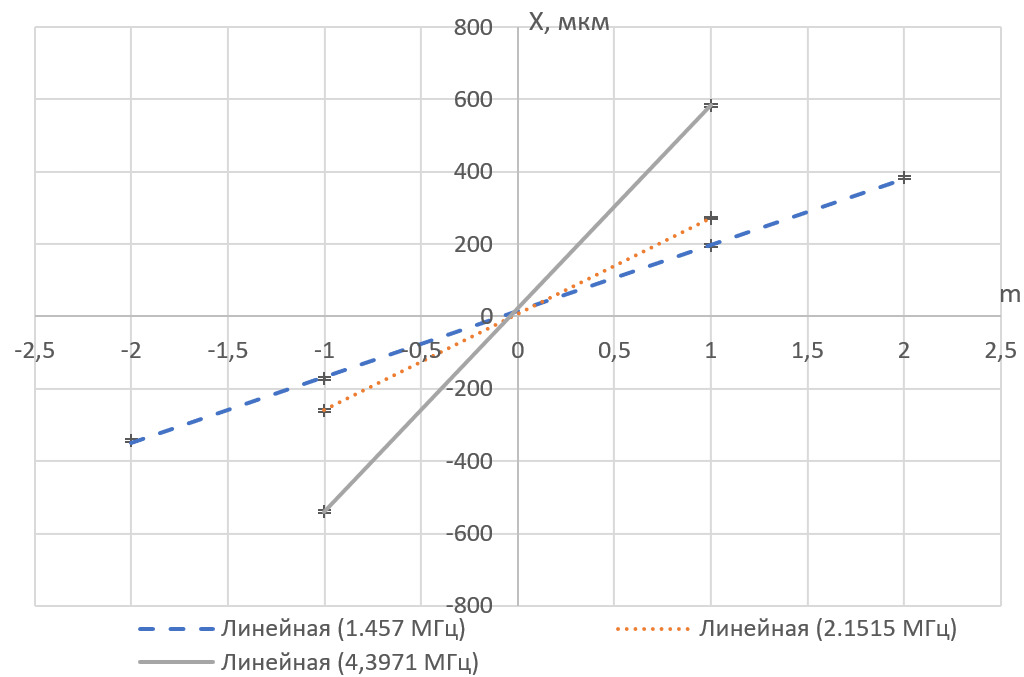
\includegraphics[width = 0.55\textwidth]{images/Im1.jpg}
		        \caption{Графики зависимости положения дифракционных максимумов от их порядка}
			\end{center}
    \end{figure}

\subsection{Исследование методом тёмного поля}


Цена деления шкалы микроскопа определяется как $$1 \;\;\text{дел} = 45 \;\;\text{мкм}.$$ Найдём длину ультразвуковой волны. Результаты измерений в таблице 3. Откуда получим $$v = 1419 \pm 40 \;\; \text{м/с}.$$

\begin{figure}[!ht]
			\begin{center}
				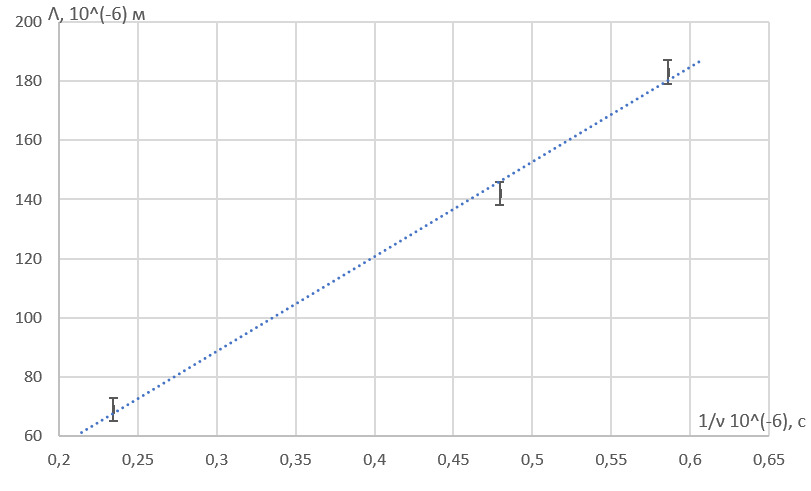
\includegraphics[width = 0.55\textwidth]{images/Im2.jpg}
		        \caption{Графики зависимости длины УЗ волны от периода}
			\end{center}
\end{figure}

\begin{table}[!ht]
    \centering
    \caption{Результат измерения длин волн}
    \begin{tabular}{|c|c|c|c|}
    \hline
    $\nu$, Мгц     & $1,7070$ & $2,0866$ & $4,2673$ \\ \hline
    $n$, дел       & $65$     & $44$     & $43$     \\ \hline
    $m$, линий     & $8$      & $7$      & $14$     \\ \hline
    $\Lambda$, мкм & $183$    & $142$    & $69$     \\ \hline
    \end{tabular}
\end{table}

\section{Вывод}

\noindent В работе не удалось провести достаточное количество измерений и получить достаточно чёткие полосы. В основном это связано с особенностями оборудования, применяемого в опыте --- генератором частот. \medskip

\noindent Так или иначе, удалось с неплохой точностью измерить скорость звука в воде используя волны как синусоидальную решётку. Кроме того, была изучена дифракция света на акустической решётке, был применён и изучен метод тёмного поля в наблюдении фазовых объектов.

\end{document}
